\chapter{参数学习}
\label{chap:pgm-parameter-learning}

在设备故障模型$F\to H\to A\leftarrow S$中，图告诉我们怎样组织故障、过热、报警和传感器失灵之间的概率关系，却没有告诉我们故障率是多少。此前的推断问题把这些概率视为已知；现在给定一批设备记录，要反过来确定它们。若应测字段都已记录且模型不含潜变量，某些参数可以通过计数或回归得到；只要模型主动引入了未观测状态，或者应测字段实际漏记，学习就可能需要在参数更新中调用推断。

本章固定图结构和局部分布的形式，沿两条彼此交叉的轴组织参数学习。数据可见性轴区分观测完整且不含潜变量、观测完整但含潜变量，以及观测字段发生缺失；估计方式轴区分输出一个参数点与保留参数后验分布。图的因子组织和归一化范围决定即使没有未观测变量时需要什么计算，未观测变量又决定是否必须恢复后验统计量。分清这些对象，才能判断算法实际优化或近似了什么，以及所得结果保留了哪种不确定性。

\section{参数学习的定义}
\label{sec:pgm-parameter-learning-definition}

设$\mathcal{G}=(V,E)$为固定图，$d=|V|$。把全部节点随机变量记为$\bm{W}=(W_1,\ldots,W_d)^\top$，并按观测状态拆成数据字段$\bm{X}$与模型主动设置的潜变量$\bm{Z}$，即在固定排列下$\bm{W}=(\bm{X}^\top,\bm{Z}^\top)^\top$。局部条件分布或势函数由参数向量$\bm{\theta}\in\Theta$控制。这里$\Theta$不仅规定参数维度，还包括概率和为$1$、方差为正、配分函数有限等约束。\term{参数学习}（parameter learning）是在这一模型族内，利用记录确定参数点或参数后验的过程；图的边是否存在、潜变量有哪些以及局部分布属于哪一族，在本章均先行确定。

\term{观测变量}（observed variable）是在当前数据获取设计中直接记录的模型变量，\term{潜变量}（latent variable）则是模型为了表达未观测状态而主动引入的随机量。\term{缺失值}（missing value）不是另一类随机变量，而是本应观测的数据字段在某条记录中没有取得的取值。参数$\bm{\theta}$控制这些变量的分布；在MLE与MAP中它是未知但固定的优化量，在分布估计中才通过先验和后验表示其不确定性。变量的观测状态、数据单元是否缺失与参数是否未知，因而是三个不同问题。

本章所说\term{观测完整}，只表示$\bm{X}$中按设计应观测的字段没有缺失，不表示模型中的每个随机变量都可见。由此，观测完整且不含潜变量时，每条记录给出全部模型变量；观测完整但含潜变量时，$\bm{X}$没有漏记，$\bm{Z}$仍按模型设定不可见；观测缺失时，$\bm{X}$还要按实际缺失模式拆成已观测部分与缺失部分。潜变量与缺失部分在计算上都要被求和或积分，但只有缺失部分还要求解释记录为何没有取得。

以观测完整且不含潜变量的独立记录为例，数据集记为$\mathcal{D}=\{\bm{x}_j\}_{j=1}^n$，其中$x_{j,i}$是第$j$条记录中节点$i$的取值。默认不同记录在给定共同参数后独立同分布，因而$p_{\bm{\theta}}(\mathcal{D})=\prod_jp_{\bm{\theta}}(\bm{x}_j)$。这不要求一条记录内部的节点独立；图模型恰好用来描述这种内部依赖。若记录是同一台设备的连续时间观测，不能直接当作独立样本，须用第~\ref{chap:pgm-dynamic}章的序列模型或另行处理时间相关性。

局部分布不同，不意味着其参数一定各自独立。\term{参数共享}（parameter sharing）让多个节点或多条记录使用同一个未知参数，例如同型号传感器共用误报率。固定图结构并未排除共享；共享参数必须同时接受所有相关局部项的约束，不能在每个节点上分别估计出不同的数再直接拼接。

要比较候选参数，需要先选定目标。\term{最大似然估计}（maximum likelihood estimation, MLE）选择使已经观测到的数据最可能的参数；\term{最大后验估计}（maximum a posteriori estimation, MAP）还利用参数先验，选择后验密度最大的点。令$\ell(\bm{\theta})=\log p_{\bm{\theta}}(\mathcal{D})$，在最优解存在时，
\begin{equation}
  \begin{aligned}
    \widehat{\bm{\theta}}_{\mathrm{ML}}
      &\in\argmax_{\bm{\theta}\in\Theta}\ell(\bm{\theta}),\\
    \widehat{\bm{\theta}}_{\mathrm{MAP}}
      &\in\argmax_{\bm{\theta}\in\Theta}
        \{\ell(\bm{\theta})+\log p(\bm{\theta})\}.
  \end{aligned}
  \label{eq:pgm-parameter-learning-point-objectives}
\end{equation}
这里似然是固定数据后关于参数的函数，不是参数的概率分布。MAP的密度及其众数相对于所选参数坐标和基准测度定义，换用非线性参数化时不能忽略Jacobian。最大值也未必唯一，甚至可能只有上确界。

MLE与MAP都只返回目标的一个最优参数点。MAP虽然使用先验，却不等于保留参数不确定性。若数据不足以排除多组参数，\term{基于分布估计的参数学习}则保留
\begin{equation}
  p(\bm{\theta}\mid\mathcal{D})
  =\frac{p_{\bm{\theta}}(\mathcal{D})p(\bm{\theta})}
  {\int_\Theta p_{\bm{\vartheta}}(\mathcal{D})
    p(\bm{\vartheta})\,\mathrm{d}\bm{\vartheta}},
  \label{eq:pgm-parameter-learning-parameter-posterior}
\end{equation}
即按照先验与数据为不同参数分配后验权重，前提是分母有限且为正。这里保留的是参数$\bm{\theta}$的后验，不是固定参数下模型变量$\bm{X},\bm{Z}$的后验；后者在含未观测变量时只是完成参数学习所需的推断对象。后验均值$\mathbb{E}[\bm{\theta}\mid\mathcal{D}]$在相应平方损失下是一个贝叶斯点估计，但它通常既不是MLE，也不是MAP，更不等于整个后验。

估计准则还要与预测对象对应。把一条记录分成输入$\bm{x}_j$与输出$\bm{y}_j$后，联合训练与条件训练分别使用
\[
  \begin{aligned}
    \ell_{\mathrm{joint}}(\bm{\theta})
      &=\sum_j\log p_{\bm{\theta}}(\bm{x}_j,\bm{y}_j),\\
    \ell_{\mathrm{cond}}(\bm{\theta})
      &=\sum_j\log p_{\bm{\theta}}(\bm{y}_j\mid\bm{x}_j).
  \end{aligned}
\]
前者同时约束输入和输出的分布；后者把输入当作给定条件，不要求为输入建立概率模型。这一区别与有向或无向的因子组织不是同一个分类维度。若两种训练共用某个联合模型的参数，由于
\[
  \log p_{\bm{\theta}}(\bm{x},\bm{y})
  =\log p_{\bm{\theta}}(\bm{y}\mid\bm{x})
   +\log p_{\bm{\theta}}(\bm{x}),
\]
两种目标一般会选择不同的参数。第~\ref{sec:pgm-parameter-learning-complete}至\ref{sec:pgm-parameter-learning-incomplete}节先沿数据可见性轴讨论MLE与MAP点估计，第~\ref{sec:pgm-parameter-learning-bayesian}节再沿分布估计轴说明怎样保留$p(\bm{\theta}\mid\mathcal{D})$；这两条轴可以组合，而不是前后互斥的学习阶段\scite{pgm-koller2009}

\section{观测完整且不含潜变量的参数学习}
\label{sec:pgm-parameter-learning-complete}

本节固定所有模型变量都已观测，比较三类图模型的MLE与MAP点估计。区别不在于数据是否完整，而在于因子怎样组织及概率对什么对象归一化：有向图的节点条件分布逐个局部归一化，联合无向图的势函数乘积对全部模型变量全局归一化，条件无向图则在每个给定输入下只对输出变量归一化。

\subsection{有向图模型}
\label{sec:pgm-parameter-learning-directed}

对有向图，联合分布已经写成局部条件分布的乘积。因此，把乘积取对数，再对样本求和，就得到
\begin{equation}
  \begin{aligned}
    \ell(\bm{\theta})
      &=\sum_{j=1}^n\sum_{i=1}^d
        \log p_{\bm{\theta}_i}
        (x_{j,i}\mid\bm{x}_{j,\operatorname{pa}(i)})\\
      &=\sum_{i=1}^d\ell_i(\bm{\theta}_i).
  \end{aligned}
  \label{eq:pgm-parameter-learning-dag-likelihood}
\end{equation}
若不同节点的参数块没有共享约束，且$\Theta=\prod_i\Theta_i$，最大化每个$\ell_i$就能最大化总似然。这个结论来自目标的可加性和参数空间的可分离性，两者缺一不可。父节点之间即使相关，也不妨碍在本节所有节点均已观测的条件下，利用它们的实测取值拟合子节点。

对离散节点，\term{条件概率表}（conditional probability table, CPT）逐行列出每种父节点配置下的子节点分布。设$X_i$有$r_i$个状态，以$a$索引其父节点的取值配置。用$\theta_{i,a,k}$表示该配置下$X_i=k$的条件概率，约束为$\theta_{i,a,k}\geq0$及$\sum_k\theta_{i,a,k}=1$。把相同局部事件的出现次数归并，得到
\begin{equation}
  \begin{aligned}
    N_{i,a,k}
      &=\sum_{j=1}^n
        \mathbf{1}\{x_{j,i}=k,\,
          \bm{x}_{j,\operatorname{pa}(i)}=a\},\\
    N_{i,a}&=\sum_{k=1}^{r_i}N_{i,a,k},\qquad
    \ell_i=\sum_a\sum_{k=1}^{r_i}
      N_{i,a,k}\log\theta_{i,a,k}.
  \end{aligned}
  \label{eq:pgm-parameter-learning-counts}
\end{equation}
这些计数是当前局部模型的\term{充分统计量}（sufficient statistic）：给定它们以后，原始记录的排列不再影响关于参数的似然。根节点只有一个空的父配置，其计数就是通常的类别频数。

固定一行$a$，在内部解上加入约束项$\lambda(1-\sum_k\theta_{i,a,k})$。对$\theta_{i,a,k}$求导得到$N_{i,a,k}/\theta_{i,a,k}=\lambda$，再对$k$求和得到$\lambda=N_{i,a}$。允许零计数对应边界解，并约定$0\log0=0$，可得
\begin{equation}
  \widehat{\theta}_{i,a,k,\mathrm{ML}}
    =\frac{N_{i,a,k}}{N_{i,a}},\qquad N_{i,a}>0.
  \label{eq:pgm-parameter-learning-cpt-mle}
\end{equation}
若$N_{i,a}=0$，该行的似然为常数，数据不能识别其概率，$0/0$不是估计值。若强制所有概率严格为正，某些含零计数的行可能只有趋近边界的上确界，而没有内部MLE。

少量记录中的零频数并不意味着某事件永远不可能发生。对每行引入\term{狄利克雷先验}（Dirichlet prior），即在概率单纯形上为整行概率分配先验权重：
\[
  p(\bm{\theta}_{i,a})
  \propto\prod_{k=1}^{r_i}
    \theta_{i,a,k}^{\alpha_{i,a,k}-1},
  \qquad \alpha_{i,a,k}>0.
\]
把对数先验加入局部对数似然，仍可逐行求MAP。记$\alpha_{i,a,0}=\sum_k\alpha_{i,a,k}$；当所有$\alpha_{i,a,k}+N_{i,a,k}>1$时，内部众数为
\begin{equation}
  \widehat{\theta}_{i,a,k,\mathrm{MAP}}
    =\frac{N_{i,a,k}+\alpha_{i,a,k}-1}
            {N_{i,a}+\alpha_{i,a,0}-r_i}.
  \label{eq:pgm-parameter-learning-cpt-map}
\end{equation}
若条件不满足，应另行分析边界和众数是否唯一，不能照套公式。特别地，均匀狄利克雷先验的内部MAP与MLE相同；常说的“加一平滑”对应后验均值，不是该先验的MAP，完整后验及后验均值留到第~\ref{sec:pgm-parameter-learning-conjugacy}节。

下面的设备记录用于连接后续计算。它们是人工构造的数据，不是实际设备统计，也不要求样本频率等于前面章节给定的教学概率。表~\ref{tab:pgm-parameter-learning-device-counts}列出$20$条完整记录在$(F,H)$上的边缘计数；$A,S$的记录不参与这里展示的两个局部参数块。

\begin{table}[htbp]
  \centering
  \begin{tabular}{lrrr}
    \toprule
    故障状态 & $H=1$ & $H=0$ & 合计\\
    \midrule
    $F=1$ & $4$ & $1$ & $5$\\
    $F=0$ & $2$ & $13$ & $15$\\
    \midrule
    合计 & $6$ & $14$ & $20$\\
    \bottomrule
  \end{tabular}
  \caption{人工构造的局部计数，所有观测字段均无缺失。每列与每行都有明确分母，可分别复核根节点故障率和给定故障状态的过热率。}
  \label{tab:pgm-parameter-learning-device-counts}
\end{table}

由计数可得$\widehat p(F=1)=5/20=0.25$，而$\widehat p(H=1\mid F=1)=4/5=0.8$、$\widehat p(H=1\mid F=0)=2/15$。若只对故障率$\pi=p(F=1)$使用$\operatorname{Beta}(2,2)$先验，即二元狄利克雷先验，则MLE为$1/4$，MAP为$6/22=3/11\approx0.2727$。先验改变了点估计目标；它怎样产生完整参数后验以及为何后验均值又不同，将在第~\ref{sec:pgm-parameter-learning-conjugacy}节回到同一组计数。

连续节点也能利用局部分解。对线性高斯条件分布，设父节点数为$m_i$，将截距与父节点组成$\bm{u}_{j,i}=(1,\bm{x}_{j,\operatorname{pa}(i)}^\top)^\top$，并令
\[
  X_i\mid\bm{X}_{\operatorname{pa}(i)}
  \sim\mathcal{N}(\bm{\beta}_i^\top\bm{u}_i,\sigma_i^2).
\]
去掉与参数无关的常数，局部负对数似然为
\[
  -\ell_i
  =\frac{n}{2}\log\sigma_i^2+
    \frac{1}{2\sigma_i^2}
      \sum_{j=1}^n(x_{j,i}-\bm{\beta}_i^\top\bm{u}_{j,i})^2.
\]
将$\bm{u}_{j,i}^\top$按样本顺序堆叠为设计矩阵$\bm{U}_i$，它有$n$行、$m_i+1$列。响应向量为$\bm{y}_i=(x_{1,i},\ldots,x_{n,i})^\top$。固定正方差，对回归系数求导得到正规方程；在$\bm{U}_i$列满秩且残差平方和为正时，
\begin{equation}
  \begin{aligned}
    \widehat{\bm{\beta}}_i
      &=(\bm{U}_i^\top\bm{U}_i)^{-1}\bm{U}_i^\top\bm{y}_i,\\
    \widehat{\sigma}_i^2
      &=\frac{1}{n}
        \lVert\bm{y}_i-\bm{U}_i\widehat{\bm{\beta}}_i\rVert_2^2.
  \end{aligned}
  \label{eq:pgm-parameter-learning-gaussian-mle}
\end{equation}
MLE方差的分母是$n$，不是用于无偏残差方差估计的$n-m_i-1$。设计矩阵秩亏时系数可能不唯一；残差全为零且方差可以任意趋近$0$时，似然无界。数值求解宜用QR等分解而不显式求逆。至此，完整有向模型的学习化成了各节点的计数或回归，困难主要在局部数据是否充足、参数是否受共享约束，而不在全局推断。

\subsection{联合无向图}
\label{sec:pgm-parameter-learning-undirected}

无向模型的势函数也分布在局部，但它们并不各自归一化。考虑固定支持集$\mathcal{X}$上的正指数族模型
\begin{equation}
  \begin{aligned}
    p_{\bm{\theta}}(\bm{x})
      &=h(\bm{x})
        \exp\{\bm{\theta}^\top\bm{T}(\bm{x})-A(\bm{\theta})\},\\
    A(\bm{\theta})&=\log Z(\bm{\theta}),\\
    Z(\bm{\theta})
      &=\int_{\mathcal{X}}h(\bm{x})
        e^{\bm{\theta}^\top\bm{T}(\bm{x})}\,\mathrm{d}\mu(\bm{x}).
  \end{aligned}
  \label{eq:pgm-parameter-learning-exponential-model}
\end{equation}
$\bm{T}$收集团上的充分统计量，$h$是与参数无关的基准因子，$\mu$在离散情形取计数测度，在连续情形取相应基准测度。要求$0<Z(\bm{\theta})<\infty$。令$\overline{\bm{T}}=n^{-1}\sum_j\bm{T}(\bm{x}_j)$，平均对数似然中与参数有关的部分为$\bm{\theta}^\top\overline{\bm{T}}-A(\bm{\theta})$。

为什么局部势的变化会引入全局计算？在可以交换微分与积分的条件下，对归一化项求导得到
\begin{equation}
  \begin{aligned}
    \nabla_{\bm{\theta}} A(\bm{\theta})
      &=\frac{1}{Z(\bm{\theta})}
        \int h(\bm{x})e^{\bm{\theta}^\top\bm{T}(\bm{x})}
             \bm{T}(\bm{x})\,\mathrm{d}\mu(\bm{x})\\
      &=\mathbb{E}_{p_{\bm{\theta}}}[\bm{T}(\bm{X})],\\
    \frac{1}{n}\nabla_{\bm{\theta}}\ell(\bm{\theta})
      &=\overline{\bm{T}}
        -\mathbb{E}_{p_{\bm{\theta}}}[\bm{T}(\bm{X})].
  \end{aligned}
  \label{eq:pgm-parameter-learning-moment-gradient}
\end{equation}
有限离散支持下可逐项求导；连续情形可由参数邻域内的可积支配函数等正则条件保证交换。梯度比较了数据实际呈现的统计量与模型预期的统计量：模型对某种相互作用估计不足，就提高它的权重；估计过多，就降低权重。最优内部点满足矩匹配，但数据矩落在可实现矩集合的边界时，有限参数MLE可能不存在。

再求一次导数，得到$\nabla^2A=\operatorname{Cov}_{p_{\bm{\theta}}}[\bm{T}(\bm{X})]$，所以线性自然参数下的对数似然是凹函数。充分统计量若有冗余，协方差可能奇异，凹性并不保证参数唯一。这一几何性质不能照搬到任意神经网络势函数的参数上；非线性参数化一般会改变优化问题的曲率。指数族与矩匹配的关系可回顾第~\ref{chap:pgm-variational}章\scite{pgm-wainwright2008}

一个只有两个节点的例子可以直接核验梯度。设$X_1,X_2\in\{-1,1\}$，$p_\theta(x_1,x_2)\propto e^{\theta x_1x_2}$。同号和异号各有两个配置，因此$Z(\theta)=2e^\theta+2e^{-\theta}=4\cosh\theta$，模型期望为$\mathbb{E}_\theta[X_1X_2]=\tanh\theta$。若$10$条记录中有$8$条同号、$2$条异号，则经验统计量为$0.6$，平均似然梯度为$0.6-\tanh\theta$。令它为零，得到$\widehat\theta=\operatorname{arctanh}(0.6)=\log2$；代回模型，同号概率$e^\theta/(e^\theta+e^{-\theta})=0.8$，恰好匹配记录。

这个例子只有四种状态，可以枚举。一般图上，直接计算$Z$或模型期望可能需要高维求和；计算梯度不一定要显式给出$Z$的数值，却仍要完成同等重要的概率推断。处理这一困难时，必须区分保留似然但近似计算，与改变学习准则。

保留似然的路线以式~\eqref{eq:pgm-parameter-learning-moment-gradient}为出发点。用MCMC产生近似服从$p_{\bm{\theta}}$的样本，再用样本均值估计模型期望；链混合不足带来偏差，样本相关性降低有效样本量。也可以通过变分推断取得近似边缘分布，计算所需的局部统计量。若使用的是某个近似对数配分函数$\widetilde A$的梯度，实际优化的便是$\bm{\theta}^\top\overline{\bm{T}}-\widetilde A(\bm{\theta})$。仅把任意近似边缘塞进梯度，并不自动保证它是某个一致目标的梯度，更没有精确似然单调增加的保证。

另一条路线主动更换准则。\term{伪似然}（pseudolikelihood）把每个节点在其余节点已知时的条件概率相乘，用一组容易归一化的预测问题替代联合密度拟合。沿用第~\ref{sec:pgm-undirected-local}节的邻居集合$N(i)$，正无向模型满足
\begin{equation}
  \ell_{\mathrm{PL}}(\bm{\theta})
  =\sum_{j=1}^n\sum_{i=1}^d
    \log p_{\bm{\theta}}
      (x_{j,i}\mid\bm{x}_{j,N(i)}).
  \label{eq:pgm-parameter-learning-pseudolikelihood}
\end{equation}
固定邻居后，不含$i$的势函数与全局$Z$一起约掉，只需对$X_i$归一化。二值节点只涉及两个候选值，因此常比全局求和容易。不过，这些条件概率的乘积一般不是原数据的联合概率，不能把伪似然值当作联合预测对数似然报告。

\term{复合似然}（composite likelihood）进一步组合若干低维边缘或条件似然，其对数形式是这些局部对数似然按固定非负权重相加，伪似然是其中一个特例。选择可计算的条件块可以避开全局归一化；若选择的边缘块本身仍难以求出，则并没有消除推断困难。在模型正确、所用局部项能够识别参数且满足通常的估计正则条件时，这类估计可以一致，但有限样本解和统计效率一般不同于MLE。其标准误也不能不加修正地套用完整似然的信息矩阵公式\scite{pgm-parameter-learning-varin2011}

若模型只给出非归一化密度，还可以把估计转化为区分数据与已知噪声的分类任务。\term{噪声对比估计}（noise-contrastive estimation, NCE）选择已知且覆盖数据支持的噪声密度$p_{\mathrm{N}}$，对每个数据样本抽取$\nu$个噪声样本，这里$\nu$为正整数。在合并后的样本中，$D=1$表示来自数据，$D=0$表示来自噪声，来源先验为$P(D=1)=1/(1+\nu)$、$P(D=0)=\nu/(1+\nu)$。若真实数据密度为$p_*$，则贝叶斯公式给出
\[
  \begin{aligned}
    P(D=1\mid\bm{x})
      &=\frac{p_*(\bm{x})P(D=1)}
        {p_*(\bm{x})P(D=1)+p_{\mathrm{N}}(\bm{x})P(D=0)}\\
      &=\frac{p_*(\bm{x})}
        {p_*(\bm{x})+\nu p_{\mathrm{N}}(\bm{x})}.
  \end{aligned}
\]
因此，分母中的$\nu$来自两类样本的数量比例。用$\widetilde p_{\bm{\theta},c}(\bm{x})=\exp\{f_{\bm{\theta}}(\bm{x})+c\}$拟合数据密度，并把负对数归一化常数作为额外标量$c$学习，就得到来源分类概率模型
\[
  a_{\bm{\theta},c}(\bm{x})
  =\frac{\widetilde p_{\bm{\theta},c}(\bm{x})}
         {\widetilde p_{\bm{\theta},c}(\bm{x})
                +\nu p_{\mathrm{N}}(\bm{x})}.
\]
$a_{\bm{\theta},c}(\bm{x})$是给定样本后“它来自数据”的概率，$\widetilde p_{\bm{\theta},c}(\bm{x})$则是待学习的数据密度形式；优化过程中后者未必已经归一化。最大化二分类对数似然
\[
  \begin{aligned}
    J_{\mathrm{NCE}}
      &=\sum_{j=1}^n\log a_{\bm{\theta},c}(\bm{x}_j)\\
      &\quad+\sum_{l=1}^{\nu n}
        \log\{1-a_{\bm{\theta},c}(\bm{y}_l)\},
        \qquad \bm{y}_l\sim p_{\mathrm{N}},
  \end{aligned}
\]
无需在每一步计算$Z$。在正确设定和可识别等条件下，NCE可以一致估计密度；这不是有限噪声样本下与MLE完全相同的目标。噪声覆盖不足或分类任务过易也会影响学习。这里的$D$只是数据与噪声的来源标签，不是原图中的待预测节点\scite{pgm-parameter-learning-gutmann2012}

对连续、光滑且正的密度，还有另一种消去归一化常数的方法。\term{分数匹配}（score matching）匹配的是数据空间中的对数密度梯度$\bm{s}_{\bm{\theta}}(\bm{x})=\nabla_{\bm{x}}\log p_{\bm{\theta}}(\bm{x})$，不是对参数求导的似然得分。由于$\log Z(\bm{\theta})$不依赖$\bm{x}$，它在这里消失。若真实密度$p_*$及模型满足可积性条件，且分部积分的边界项为零，则
\begin{equation}
  \begin{aligned}
    J_{\mathrm{SM}}(\bm{\theta})
      &=\frac12\mathbb{E}_{p_*}
          \lVert\bm{s}_{\bm{\theta}}-\nabla_{\bm{x}}\log p_*\rVert_2^2\\
      &=\mathbb{E}_{p_*}\!\left[
          \frac12\lVert\bm{s}_{\bm{\theta}}\rVert_2^2+
          \nabla_{\bm{x}}\!\cdot\bm{s}_{\bm{\theta}}
        \right]+C.
  \end{aligned}
  \label{eq:pgm-parameter-learning-score-matching}
\end{equation}
$C$与模型参数无关。关键一步是分部积分：
\[
  -\int\bm{s}_{\bm{\theta}}^\top\nabla p_*\,\mathrm{d}\bm{x}
  =\int p_*\nabla\cdot\bm{s}_{\bm{\theta}}\,\mathrm{d}\bm{x}.
\]
因此未知的真实分数从可优化部分消失，可以用训练样本均值替代期望。这一标准形式不能直接用于离散变量或边界项不消失的受限支持；它优化的是分数之间的差距，而不是直接近似似然梯度\scite{pgm-parameter-learning-hyvarinen2005}

有限步链则需要单独辨认。\term{对比散度}（contrastive divergence, CD）通常从训练样本启动以$p_{\bm{\theta}}$为平稳分布的Markov链，运行$k$步，以终点统计量替代模型期望。若经验分布为$\widehat p$、转移核为$K_{\bm{\theta}}$，则其期望更新方向为
\[
  \bm{g}_{\mathrm{CD},k}
    =\mathbb{E}_{\widehat p}[\bm{T}]
      -\mathbb{E}_{\widehat pK_{\bm{\theta}}^k}[\bm{T}].
\]
有限$k$时，$\widehat pK_{\bm{\theta}}^k$通常不同于$p_{\bm{\theta}}$，所以即使无限增加平行链数、消除了Monte Carlo波动，偏差仍可能存在。虽然名称来自两个KL散度之差，但链终点分布也依赖参数；通常更新省略了这部分导数，一般不能解释为某个固定替代目标的精确梯度。已有二值受限玻尔兹曼机的反例直接说明这一点，特殊转移核下的对应关系不应推广成一般结论\scite{pgm-parameter-learning-sutskever2010}

\term{持久链}（persistent chain）在下一次参数更新时沿用上次的链状态，避免每次都从数据重新启动。它试图在模型缓慢变化时持续跟踪模型分布，但固定的少量转移并不保证链已达到新参数下的平稳状态。充分混合的MCMC与有限步持久链使用同一个模型期望公式，区别在于后者依赖跨迭代跟踪的近似；CD还固定采用数据初始化。它们与伪似然、NCE和分数匹配的区别，则在于后几种方法明确改变了学习准则。讨论效果时，既要说明计算预算，也要说明所优化或近似的对象\scite{goodfellow2016}

\subsection{条件无向图}
\label{sec:pgm-parameter-learning-conditional}

若目标是根据已经给出的测量$\bm{x}$预测一组标签$\bm{y}$，就可以只归一化标签空间。\term{条件随机场}（conditional random field, CRF）通过局部特征组织一个条件联合分布，让多个标签在给定输入以后仍能相互依赖。在线性参数化下写为
\begin{equation}
  \begin{aligned}
    p_{\bm{\theta}}(\bm{y}\mid\bm{x})
      &=\frac{\exp\{\bm{\theta}^\top\bm{f}(\bm{x},\bm{y})\}}
              {Z_{\bm{\theta}}(\bm{x})},\\
    Z_{\bm{\theta}}(\bm{x})
      &=\sum_{\bm{y}'}
         \exp\{\bm{\theta}^\top\bm{f}(\bm{x},\bm{y}')\}.
  \end{aligned}
  \label{eq:pgm-parameter-learning-crf}
\end{equation}
特征$\bm{f}$通常是各团特征的和，可以依赖整个已知输入；图主要限制标签之间的相互作用。不同输入有不同的条件配分函数，不能把所有样本的归一化项合并成一个与输入无关的数。

对完整标签训练集$\{(\bm{x}_j,\bm{y}_j)\}_{j=1}^n$，以$\lambda\geq0$控制二次正则化，目标及梯度为
\begin{equation}
  \begin{aligned}
    J(\bm{\theta})
      &=\sum_{j=1}^n
        \left[\bm{\theta}^\top\bm{f}(\bm{x}_j,\bm{y}_j)
                    -\log Z_{\bm{\theta}}(\bm{x}_j)\right]\\
      &\quad-\frac{\lambda}{2}\lVert\bm{\theta}\rVert_2^2,\\
    \nabla_{\bm{\theta}}J
      &=\sum_{j=1}^n
        \left[\bm{f}(\bm{x}_j,\bm{y}_j)
          -\mathbb{E}_{p_{\bm{\theta}}(\bm{Y}\mid\bm{x}_j)}
             \bm{f}(\bm{x}_j,\bm{Y})\right]\\
      &\quad-\lambda\bm{\theta}.
  \end{aligned}
  \label{eq:pgm-parameter-learning-crf-gradient}
\end{equation}
推导与无向联合模型相同，只是每次都固定输入再求和。梯度要求“在这一输入下，真实标签的特征”与“模型可能预测的所有标签的平均特征”匹配。$\lambda>0$时，正则项也可解释为各参数服从方差$\lambda^{-1}$的零均值高斯先验所产生的MAP项。

例如，只有一个二元标签、一个标量特征$f(x,y)=yx$时，$p_\theta(Y=1\mid x)=\operatorname{sigmoid}(\theta x)$。单条记录$(x,y)=(2,1)$在$\theta=0$处贡献梯度$2-2\times0.5=1$，推动正类概率上升。多个相互依赖的标签使这种期望计算变复杂：线性链可以通过前向后向递推计算局部边缘，一般图则可能需要近似推断。固定特征的线性CRF具有凹的条件对数似然，但无正则化时仍可能因可分离等情形没有有限最优解；神经特征参与学习时也不再一般地凹。第~\ref{chap:pgm-energy-models}章将展开具体CRF结构及其计算。

\section{观测完整但含潜变量的参数学习}
\label{sec:pgm-parameter-learning-latent}

现在假定按设计应记录的数据字段$\bm{X}$全部可见，但模型还含有从不直接观测的潜变量$\bm{Z}$。完整观测不再提供完整模型配置，局部计数或回归矩必须由潜变量后验的期望替代。本节主要讨论MLE与MAP点估计：先写出需要优化的观测数据似然，再以精确EM、GEM、近似E步和摊销推断说明推断与参数更新怎样配合。

\subsection{观测数据似然}
\label{sec:pgm-parameter-learning-marginal-likelihood}

没有观测到$\bm{z}_j$，并不意味着可以把它设置为零或直接删除其因子。每种相容取值都可能产生当前记录，因此要按模型概率加总：
\begin{equation}
  \ell(\bm{\theta})
    =\sum_{j=1}^n\log p_{\bm{\theta}}(\bm{x}_j)
    =\sum_{j=1}^n
       \log\int p_{\bm{\theta}}(\bm{x}_j,\bm{z}_j)
                         \,\mathrm{d}\bm{z}_j.
  \label{eq:pgm-parameter-learning-observed-likelihood}
\end{equation}
离散变量把积分换成求和。这里的\term{边缘似然}（marginal likelihood）是消去潜变量之后、仍作为$\bm{\theta}$函数的观测似然；它不同于式~\eqref{eq:pgm-parameter-learning-parameter-posterior}分母中进一步积分参数所得的模型证据。前者用于本章的参数优化，后者常用于模型比较。

对数外面有求和、里面又有积分，模型配置完整时可得的局部计数不再直接可用。在微分与积分可交换、观测密度为正时，
\begin{equation}
  \begin{aligned}
    \nabla_{\bm{\theta}}\log p_{\bm{\theta}}(\bm{x}_j)
      &=\frac{\int\nabla_{\bm{\theta}}
          p_{\bm{\theta}}(\bm{x}_j,\bm{z}_j)
                  \,\mathrm{d}\bm{z}_j}
             {p_{\bm{\theta}}(\bm{x}_j)}\\
      &=\mathbb{E}_{p_{\bm{\theta}}(\bm{Z}_j\mid\bm{x}_j)}
          [\nabla_{\bm{\theta}}
            \log p_{\bm{\theta}}(\bm{x}_j,\bm{Z}_j)].
  \end{aligned}
  \label{eq:pgm-parameter-learning-fisher-identity}
\end{equation}
第二个等号使用$\nabla p=p\nabla\log p$，再将联合密度除以观测密度识别为后验。这说明直接梯度优化同样需要当前参数下的后验推断。对离散CPT，原来的事件指示量要换成“该事件在当前观测下发生的后验概率”。这个概率又依赖正在学习的参数，不能预先算一次就永久当作真实计数。

沿用表~\ref{tab:pgm-parameter-learning-device-counts}的过热总数，考虑另一种模型：数据字段只有$H$，故障状态$F$被主动设置为潜变量；$A,S$在这次教学计算中不进入模型。为了只研究一个未知量，把过热条件概率固定为另行给定的校准值$p(H=1\mid F=1)=0.8$和$p(H=1\mid F=0)=0.1$，仅学习$\pi=p(F=1)$。这里没有本应记录却漏记的$F$，也不是重新使用完整表估计两个条件概率。于是
\[
  p_\pi(H=1)=0.8\pi+0.1(1-\pi)=0.1+0.7\pi.
\]
$20$条记录中$6$条过热、$14$条不过热，观测对数似然为
\begin{equation}
  \ell(\pi)=6\log(0.1+0.7\pi)
             +14\log(0.9-0.7\pi),\qquad 0\leq\pi\leq1.
  \label{eq:pgm-parameter-learning-device-observed}
\end{equation}
它在$p_\pi(H=1)=6/20$处最大，故$\widehat\pi_{\mathrm{ML}}=2/7$。这个一维例子可以直接解出，适合用来检查EM；更复杂图中的边缘似然通常不能这样化简。若把两项过热条件概率也设为未知，单一的过热频率便不足以识别三个参数，困难就不只是如何优化了。

\subsection{精确EM}
\label{sec:pgm-parameter-learning-em}

式~\eqref{eq:pgm-parameter-learning-fisher-identity}把未知状态换成后验平均。观测量与未观测随机量合称为\term{完全数据}（complete data）；本节中它是$(\bm{X},\bm{Z})$，不表示$\bm{Z}$真的被记录下来。若给定完全数据后容易求出最优参数，我们可以进一步利用这一结构：在当前参数下算出潜变量的后验统计量，再把它们固定下来更新参数。\term{期望最大化算法}（expectation-maximization algorithm, EM）正是这样交替进行推断与优化；E步不是把每个潜变量硬选成一个最可能值，M步也不是对刚才的随机猜测重新计数。

为推导更新为何有效，对每条记录引入潜变量分布$q_j(\bm{z}_j)$。先取它在相应联合密度为正的支持上为正，并假设下式期望与熵有限。利用$\log$的凹性和Jensen不等式，
\begin{equation}
  \begin{aligned}
    \log p_{\bm{\theta}}(\bm{x}_j)
      &=\log\mathbb{E}_{q_j}
        \left[\frac{p_{\bm{\theta}}(\bm{x}_j,\bm{Z}_j)}
                    {q_j(\bm{Z}_j)}\right]\\
      &\geq
        \mathbb{E}_{q_j}\log p_{\bm{\theta}}
             (\bm{x}_j,\bm{Z}_j)+\mathcal{H}(q_j),
  \end{aligned}
  \label{eq:pgm-parameter-learning-jensen}
\end{equation}
其中$\mathcal{H}(q_j)=-\mathbb{E}_{q_j}\log q_j$，连续情形为微分熵。每条记录的右侧就是式~\eqref{eq:pgm-variational-elbo}中的$\mathcal{L}(q_j)$；这里只是显式恢复待学习的模型参数。把各条记录相加，记下界为$\mathcal{F}(q,\bm{\theta})$。更精确的关系是
\begin{equation}
  \begin{aligned}
    \mathcal{F}(q,\bm{\theta})
      &=\sum_j\{\mathbb{E}_{q_j}
          \log p_{\bm{\theta}}(\bm{x}_j,\bm{Z}_j)
                      +\mathcal{H}(q_j)\},\\
    \ell(\bm{\theta})
      &=\mathcal{F}(q,\bm{\theta})
        +\sum_j\operatorname{KL}
          \bigl(q_j\,\|\,p_{\bm{\theta}}(\bm{Z}_j\mid\bm{x}_j)\bigr).
  \end{aligned}
  \label{eq:pgm-parameter-learning-elbo-identity}
\end{equation}
第二式直接由后验密度的定义代入KL散度得到；只要$q_j$对后验绝对连续且各项有限，它也适用于$q_j$仅覆盖部分后验支持的情况。这就是本章使用的\term{证据下界}（evidence lower bound, ELBO）：它的下界对象是当前参数下的观测对数似然。KL散度非负，并且在$q_j$等于真实后验时为零，因此这个下界可以在当前参数处与似然相等。

固定第$t$次参数$\bm{\theta}^{(t)}$，E步取
\[
  q_j^{(t)}(\bm{z}_j)
    =p_{\bm{\theta}^{(t)}}(\bm{z}_j\mid\bm{x}_j).
\]
随后固定这些分布，定义
\begin{equation}
  \begin{aligned}
    Q(\bm{\theta}\mid\bm{\theta}^{(t)})
      &=\sum_j\mathbb{E}_{q_j^{(t)}}
          \log p_{\bm{\theta}}(\bm{x}_j,\bm{Z}_j),\\
    \bm{\theta}^{(t+1)}
      &\in\argmax_{\bm{\theta}\in\Theta}
         Q(\bm{\theta}\mid\bm{\theta}^{(t)}).
  \end{aligned}
  \label{eq:pgm-parameter-learning-em-update}
\end{equation}
熵在M步中不依赖新参数，所以最大化$Q$等价于最大化固定$q^{(t)}$的下界。这里必须区分积分所用的旧参数与被优化的新参数；若在M步里随意重算$q$，就不再是这个固定下界的优化。

\begin{theorem}[EM的观测似然单调性]
  \label{thm:pgm-parameter-learning-em-monotonicity}
  设$\bm{x}_1,\ldots,\bm{x}_n$为固定观测，$\bm{Z}_j$为第$j$条记录的潜变量。对每个$j$，分别在观测空间和潜变量空间上给定$\sigma$有限基准测度$\nu_j$与$\mu_j$；对每个$\bm{\theta}\in\Theta$，$p_{\bm{\theta}}(\bm{x},\bm{z})$是相对于共同乘积测度$\nu_j\otimes\mu_j$的联合密度。有限离散情形取计数测度，此时该密度就是联合概率质量函数。定义观测边缘密度，并在该边缘正且有限时定义后验密度：
  \[
    \begin{aligned}
      p_{\bm{\theta}}(\bm{x}_j)
        &\mathrel{:=}\int
          p_{\bm{\theta}}(\bm{x}_j,\bm{z})\,
          \mathrm{d}\mu_j(\bm{z}),\\
      r_{j,\bm{\theta}}(\bm{z}\mid\bm{x}_j)
        &\mathrel{:=}
          \frac{p_{\bm{\theta}}(\bm{x}_j,\bm{z})}
               {p_{\bm{\theta}}(\bm{x}_j)},\\
      \ell(\bm{\theta})
        &\mathrel{:=}\sum_{j=1}^n
          \log p_{\bm{\theta}}(\bm{x}_j).
    \end{aligned}
  \]
  取$\bm{\theta}^{(t)},\bm{\theta}^{(t+1)}\in\Theta$，假设对$s\in\{t,t+1\}$及每个$j$都有$0<p_{\bm{\theta}^{(s)}}(\bm{x}_j)<\infty$。E步精确取$q_j^{(t)}(\bm{z})=r_{j,\bm{\theta}^{(t)}}(\bm{z}\mid\bm{x}_j)$，并定义
  \[
    Q(\bm{\theta}\mid\bm{\theta}^{(t)})
      \mathrel{:=}\sum_{j=1}^n\int
        q_j^{(t)}(\bm{z})
        \log p_{\bm{\theta}}(\bm{x}_j,\bm{z})\,
        \mathrm{d}\mu_j(\bm{z}).
  \]
  假设对每个$j$及$s\in\{t,t+1\}$，都有
  \[
    \int q_j^{(t)}(\bm{z})
      \log p_{\bm{\theta}^{(s)}}(\bm{x}_j,\bm{z})\,
      \mathrm{d}\mu_j(\bm{z})\in\mathbb{R},
  \]
  并且
  \[
    \operatorname{KL}\!\left(
      q_j^{(t)}\,\middle\|\,
      r_{j,\bm{\theta}^{(t+1)}}(\,\cdot\mid\bm{x}_j)
    \right)
    \mathrel{:=}\int q_j^{(t)}(\bm{z})
      \log\frac{q_j^{(t)}(\bm{z})}
                    {r_{j,\bm{\theta}^{(t+1)}}(\bm{z}\mid\bm{x}_j)}
      \,\mathrm{d}\mu_j(\bm{z})
    <\infty,
  \]
  其中不满足绝对连续时按惯例令KL散度为$+\infty$。若新参数满足
  \[
    Q(\bm{\theta}^{(t+1)}\mid\bm{\theta}^{(t)})
    \geq Q(\bm{\theta}^{(t)}\mid\bm{\theta}^{(t)}),
  \]
  则$\ell(\bm{\theta}^{(t+1)})\geq\ell(\bm{\theta}^{(t)})$。
\end{theorem}

\begin{proof}
  由$q_j^{(t)}=r_{j,\bm{\theta}^{(t)}}(\,\cdot\mid\bm{x}_j)$及后验密度的定义，对$q_j^{(t)}$几乎处处有
  \[
    \log\frac{q_j^{(t)}(\bm{z})}
                  {r_{j,\bm{\theta}^{(t+1)}}(\bm{z}\mid\bm{x}_j)}
    =
    \log\frac{p_{\bm{\theta}^{(t)}}(\bm{x}_j,\bm{z})}
                  {p_{\bm{\theta}^{(t+1)}}(\bm{x}_j,\bm{z})}
    +\log\frac{p_{\bm{\theta}^{(t+1)}}(\bm{x}_j)}
                   {p_{\bm{\theta}^{(t)}}(\bm{x}_j)}.
  \]
  定理中的有限性条件允许对该等式积分并重排有限项。逐个$j$相加得到
  \[
    \begin{aligned}
      \ell(\bm{\theta}^{(t+1)})-\ell(\bm{\theta}^{(t)})
      &=
      Q(\bm{\theta}^{(t+1)}\mid\bm{\theta}^{(t)})\\
      &\quad-Q(\bm{\theta}^{(t)}\mid\bm{\theta}^{(t)})\\
      &\quad+\sum_{j=1}^n
        \operatorname{KL}\!\left(
          q_j^{(t)}\,\middle\|\,
          r_{j,\bm{\theta}^{(t+1)}}(\,\cdot\mid\bm{x}_j)
        \right).
    \end{aligned}
  \]
  右侧的$Q$函数之差由假设非负，各KL散度也非负，因此观测对数似然不下降。
\end{proof}

这个证明只依赖下界在旧点精确贴合，以及同一下界在M步得到改进。它没有证明找到全局最大值，也没有证明每次严格增加；即使似然值收敛，参数序列的收敛和极限点性质仍需额外条件。EM的原始论文给出了含未观测量的数据学习框架，而下界视角清楚展示了哪些更新仍保留上述论证\scite{pgm-overview-dempster1977}

对离散有向图，E步实际需要的是各节点家庭的后验边缘，而不必显式列出整个联合后验。沿用章首覆盖全部图节点的$\bm{W}=(\bm{X}^\top,\bm{Z}^\top)^\top$，将式~\eqref{eq:pgm-parameter-learning-counts}中的计数替换为
\begin{equation}
  \overline N_{i,a,k}^{(t)}
    =\sum_{j=1}^n
      p_{\bm{\theta}^{(t)}}\!
        \left(W_i=k,\bm{W}_{\operatorname{pa}(i)}=a
                    \mid\bm{X}=\bm{x}_j\right),
  \label{eq:pgm-parameter-learning-expected-counts}
\end{equation}
这里$\bm{x}_j$是第$j$条完整观测记录；若节点$i$或其父节点中含有潜变量，条件概率便对这些未观测取值求后验平均。M步将每行期望计数归一化，即$\theta_{i,a,k}^{(t+1)}=\overline N_{i,a,k}^{(t)}/\sum_l\overline N_{i,a,l}^{(t)}$，分母为正时成立。期望计数可以是小数；其含义是当前模型给各节点家庭事件分配的总后验权重。对高斯局部模型，所需的是潜变量的一阶矩、二阶矩和交叉乘积期望；只把潜变量替换成后验均值会丢掉条件方差，通常不是正确的E步。

\begin{algorithm}[利用后验充分统计量的EM]
  \label{alg:pgm-parameter-learning-em}
  \begin{algorithmic}[1]
    \Require 观测数据、固定联合模型、可行初值$\bm{\theta}^{(0)}$、容差$\varepsilon>0$和迭代上限
    \Ensure 参数估计及观测对数似然的迭代记录
    \For{$t=0,1,\ldots$，直到达到迭代上限}
      \State 对各记录在$\bm{\theta}^{(t)}$下作后验推断，聚合所需充分统计量
      \State 固定这些统计量，最大化$Q(\bm{\theta}\mid\bm{\theta}^{(t)})$，得到$\bm{\theta}^{(t+1)}$
      \State 计算$\Delta_t=\ell(\bm{\theta}^{(t+1)})-\ell(\bm{\theta}^{(t)})$
      \If{$0\leq\Delta_t\leq\varepsilon(1+|\ell(\bm{\theta}^{(t)})|)$}
        \State 停止迭代并返回当前参数
      \EndIf
    \EndFor
  \end{algorithmic}
\end{algorithm}

算法~\ref{alg:pgm-parameter-learning-em}的停止判据要求能够可靠计算观测似然。若$\Delta_t$超出数值容差地为负，应检查推断、M步和数值实现；不能把它当成精确EM的正常现象。无法精确评估似然时，需要另行报告所监测的近似目标与误差，不能把近似停止条件解释为已经验证精确单调性。

\begin{example}[由过热记录学习故障率]
  \label{ex:pgm-parameter-learning-device-em}
  使用式~\eqref{eq:pgm-parameter-learning-device-observed}的$6$条过热、$14$条不过热记录，并从$\pi^{(0)}=0.1$出发。E步分别计算
  \[
    \begin{aligned}
      r_1&=p(F=1\mid H=1)
        =\frac{0.1\times0.8}{0.1\times0.8+0.9\times0.1}
        =\frac{8}{17},\\
      r_0&=p(F=1\mid H=0)
        =\frac{0.1\times0.2}{0.1\times0.2+0.9\times0.9}
        =\frac{2}{83}.
    \end{aligned}
  \]
  故障期望计数为$6r_1+14r_0=4460/1411\approx3.1609$，不是$6$，也不是把每条记录硬分配后得到的整数。M步最大化
  \[
    \begin{aligned}
      Q(\pi\mid\pi^{(0)})
        &=(6r_1+14r_0)\log\pi\\
        &\quad+(20-6r_1-14r_0)\log(1-\pi)+C,
    \end{aligned}
  \]
  因而$\pi^{(1)}=(6r_1+14r_0)/20=223/1411\approx0.158044$。用自然对数代回观测似然，有$\ell(\pi^{(0)})\approx-13.240355$、$\ell(\pi^{(1)})\approx-12.657187$。再做一轮得到$\pi^{(2)}\approx0.208111$、$\ell(\pi^{(2)})\approx-12.369507$；直接求得的最优值为$\ell(2/7)\approx-12.217286$。
\end{example}

图~\ref{fig:pgm-parameter-learning-em-bound}显示第一轮的几何关系。M步最大化的是旧后验构造的下界，不是一步直接跳到观测似然的峰值；新参数处下界与似然之间的间隙，会在下一次精确E步中被补齐。这个差别解释了为何一个已能直接求解的一维问题，EM仍可能需要多轮更新。

\begin{figure}[htbp]
  \centering
  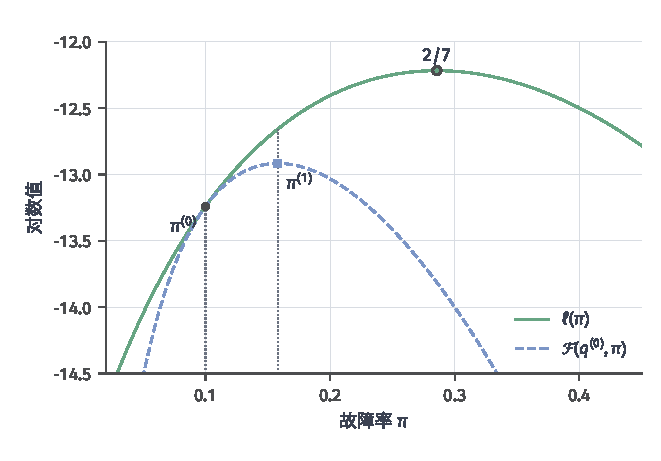
\includegraphics[width=\linewidth]{figures/03-models/03-probabilistic-graphical-models/matplotlib/pgm-parameter-learning-em-bound/figure.pdf}
  \caption{故障率例子的第一轮EM。实线是观测对数似然，虚线是固定$\pi^{(0)}=0.1$后验所得的下界。两者在旧参数处相等；下界在$\pi^{(1)}\approx0.158044$处最大，而观测似然在$2/7$处最大。图中纵轴为自然对数，曲线可由正文公式直接复算。}
  \label{fig:pgm-parameter-learning-em-bound}
\end{figure}

\begin{figure}[htbp]
  \centering
  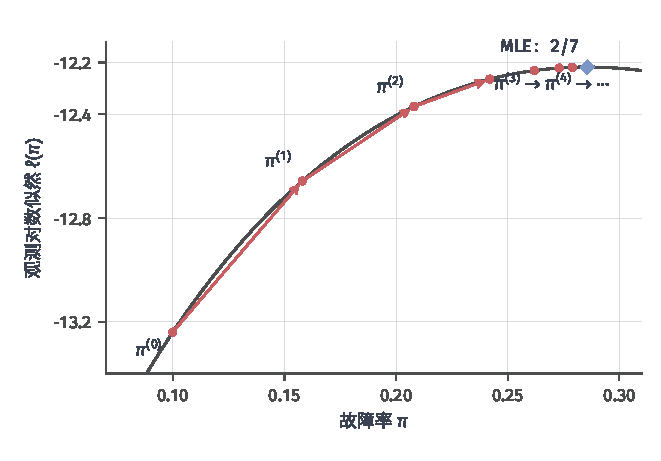
\includegraphics[width=\linewidth]{figures/03-models/03-probabilistic-graphical-models/matplotlib/pgm-parameter-learning-em-trajectory/figure.pdf}
  \caption{同一标量例子的多轮EM轨迹。红点依次为$\pi^{(0)},\ldots,\pi^{(6)}$，纵坐标均使用观测对数似然而非各轮不同的下界；蓝色菱形是解析MLE $2/7$。轨迹展示似然逐轮上升并逐渐靠近驻点，但不把这一维构造推广为一般EM的全局最优保证。}
  \label{fig:pgm-parameter-learning-em-trajectory}
\end{figure}

\subsection{广义EM与近似E步}
\label{sec:pgm-parameter-learning-em-extensions}

定理~\ref{thm:pgm-parameter-learning-em-monotonicity}并没有要求M步一定找到$Q$的全局最大值。\term{广义EM}（generalized EM, GEM）保留精确E步，只要求M步改进同一个$Q$。例如，对$Q$做带回溯检查的梯度上升，或依次改进几个参数块，只要总更新不降低$Q$，就仍能保证观测似然不下降。任意走一步梯度、未经检查地使用过大步长，并不自动满足GEM的条件。

如果后验推断本身难以完成，则可以限制$q$属于某个可计算分布族$\mathcal{Q}$。\term{变分EM}（variational EM）在$\mathcal{F}(q,\bm{\theta})$上交替改进近似后验和参数：
\begin{equation}
  \begin{aligned}
    q^{(t+1)}
      &\in\argmax_{q\in\mathcal{Q}}\mathcal{F}(q,\bm{\theta}^{(t)}),\\
    \bm{\theta}^{(t+1)}
      &\in\argmax_{\bm{\theta}\in\Theta}
         \mathcal{F}(q^{(t+1)},\bm{\theta}).
  \end{aligned}
  \label{eq:pgm-parameter-learning-variational-em}
\end{equation}
精确最大化可以放宽为保证同一目标不下降的更新。在固定数据、模型和变分族下，两步都做到这一点，便有
\[
  \mathcal{F}(q^{(t+1)},\bm{\theta}^{(t+1)})
  \geq\mathcal{F}(q^{(t)},\bm{\theta}^{(t)}).
\]
但近似后验一般不能使KL间隙为零，旧点的“下界等于似然”不再成立，所以这个结论只保证ELBO单调，不保证观测似然单调\scite{pgm-parameter-learning-neal1998}

更明确地，记$K_t=\sum_j\operatorname{KL}(q_j^{(t)}\,\|\,p_{\bm{\theta}^{(t)}}(\bm{Z}_j\mid\bm{x}_j))$，并简记$\mathcal{F}_t=\mathcal{F}(q^{(t)},\bm{\theta}^{(t)})$，则式~\eqref{eq:pgm-parameter-learning-elbo-identity}给出
\[
  \ell(\bm{\theta}^{(t+1)})-\ell(\bm{\theta}^{(t)})
  =\mathcal{F}_{t+1}-\mathcal{F}_t+K_{t+1}-K_t.
\]
即使第一项非负，后验近似间隙的变化仍可能使总和为负。随机梯度或有噪声的下界估计，还可能连逐步ELBO单调性都不具备。Monte Carlo E步用有限样本近似$Q$时，同样不能直接套用精确EM定理；需要控制采样误差并核查实际改进。

MAP也可以采用EM式更新：E步仍计算给定当前参数的潜变量后验，M步改进$Q(\bm{\theta}\mid\bm{\theta}^{(t)})+\log p(\bm{\theta})$。在对应条件下，单调对象变成$\ell(\bm{\theta})+\log p(\bm{\theta})$，即相差常数的对数后验密度，而非数据似然本身。把先验引入M步不等于保留了参数后验；这仍是点估计方法。

\subsection{摊销推断与Wake--Sleep}
\label{sec:pgm-parameter-learning-amortized}

变分EM若为每条记录分别保存$q_j$，新记录到来时还要重新求解一个局部优化问题。\term{摊销推断}（amortized inference）改用共享映射$q_{\bm{\phi}}(\bm{z}\mid\bm{x})$，由识别参数$\bm{\phi}$直接把观测映射为近似后验。对固定数据集，可以联合改进
\[
  \mathcal{F}(\bm{\theta},\bm{\phi})
  =\sum_{j=1}^n\mathbb{E}_{q_{\bm{\phi}}(\bm{Z}\mid\bm{x}_j)}
    [\log p_{\bm{\theta}}(\bm{x}_j,\bm{Z})
     -\log q_{\bm{\phi}}(\bm{Z}\mid\bm{x}_j)].
\]
共享映射减少了逐样本优化与存储，却需要分清三种不同的差距。若局部变分族$\mathcal{Q}$不包含真实后验，即使每条记录都求得族内最优$q_j^\star$，仍有由变分族限制带来的近似误差。再用共享映射$q_{\bm{\phi}}(\bm{z}\mid\bm{x})$代替这些逐样本最优解时，所选映射族的最佳结果与各$q_j^\star$之间的目标值差距才是\term{摊销误差}（amortization error），有限网络容量是其来源之一。实际训练若尚未达到该映射族内的最优$\bm{\phi}$，产生的是优化误差，不能再归入摊销误差。具体的梯度估计与重参数化方法见第~\ref{sec:pgm-variational-amortized}节。

\term{Wake--Sleep算法}由Hinton等在1995年为随机Helmholtz机提出。它同时维护自上而下的\term{生成模型}（generative model）$p_{\bm{\theta}}(\bm{x},\bm{z})$与自下而上的\term{识别模型}（recognition model）$q_{\bm{\phi}}(\bm{z}\mid\bm{x})$，但两组参数不在同一个阶段更新。Wake阶段从训练数据取得$\bm{x}$，再由识别模型抽取$\bm{z}$，固定$\bm{\phi}$并更新生成参数$\bm{\theta}$，使这些“数据--解释”对在生成模型下更可能；Sleep阶段固定$\bm{\theta}$，从生成模型自上而下抽取$(\bm{x},\bm{z})$，再更新$\bm{\phi}$，使识别模型能够从生成出的$\bm{x}$恢复对应的$\bm{z}$\scite{pgm-parameter-learning-hinton1995}

这两个方向可以写成不同的总体目标。Wake阶段关于生成参数最大化
\begin{equation}
  J_{\mathrm{wake}}(\bm{\theta};\bm{\phi})
  =\frac{1}{n}\sum_{j=1}^n
    \mathbb{E}_{q_{\bm{\phi}}(\bm{Z}\mid\bm{x}_j)}
      [\log p_{\bm{\theta}}(\bm{x}_j,\bm{Z})],
  \label{eq:pgm-parameter-learning-wake-objective}
\end{equation}
它是固定识别模型后ELBO中依赖$\bm{\theta}$的部分，近似后验的间隙方向为$\operatorname{KL}(q_{\bm{\phi}}(\bm{Z}\mid\bm{x})\,\|\,p_{\bm{\theta}}(\bm{Z}\mid\bm{x}))$。经典算法用$q_{\bm{\phi}}$的样本形成局部随机更新，并不在Wake阶段沿识别参数求这个ELBO的梯度。

Sleep阶段关于识别参数最大化
\begin{equation}
  \begin{aligned}
    J_{\mathrm{sleep}}(\bm{\phi};\bm{\theta})
      &=\mathbb{E}_{p_{\bm{\theta}}(\bm{X},\bm{Z})}
          [\log q_{\bm{\phi}}(\bm{Z}\mid\bm{X})]\\
      &=-\mathbb{E}_{p_{\bm{\theta}}(\bm{X})}
          \operatorname{KL}\bigl(
            p_{\bm{\theta}}(\bm{Z}\mid\bm{X})
            \,\|\,q_{\bm{\phi}}(\bm{Z}\mid\bm{X})\bigr)+C(\bm{\theta}),
  \end{aligned}
  \label{eq:pgm-parameter-learning-sleep-objective}
\end{equation}
其中$C(\bm{\theta})$与$\bm{\phi}$无关。这里的KL方向与Wake阶段ELBO中的方向相反，而且外层输入来自当前生成模型，不是经验数据分布。生成模型尚未覆盖真实数据的重要区域时，Sleep阶段也不会在这些区域训练识别模型。

因此，Wake--Sleep不是精确EM的另一种实现。它用摊销识别模型近似后验，Sleep阶段又优化不同方向、不同输入分布下的识别目标；随机更新还会带来抽样与优化误差。算法可以改进各阶段实际使用的目标，却没有“每轮观测数据似然必不下降”的精确EM保证，也不能把Sleep目标的改善解释为真实数据ELBO必然改善。

\section{观测缺失下的参数学习}
\label{sec:pgm-parameter-learning-incomplete}

观测缺失意味着按设计应记录的数据字段没有全部取得。缺失值与潜变量都形成未观测量，所以第~\ref{sec:pgm-parameter-learning-latent}节的边缘化和近似推断工具可以复用；但在复用之前，必须先判断记录过程是否携带了关于缺失值的额外信息。本节只建立这种映射和适用条件，不重复EM推导。

\subsection{缺失变量与缺失机制}
\label{sec:pgm-parameter-learning-missingness}

以$\bm{Y}$表示本应完整记录的数据向量，$R_i=1$表示$Y_i$已观测，$R_i=0$表示缺失。对一种固定模式$\bm{r}$，把$\bm{y}$拆为$\bm{y}_{\mathrm{obs}}$与$\bm{y}_{\mathrm{mis}}$，拆分位置由$\bm{r}$决定。数据模型为$p_{\bm{\theta}}(\bm{y})$，\term{缺失机制}（missingness mechanism）为$p_{\bm{\psi}}(\bm{r}\mid\bm{y})$，其中$\bm{\psi}$控制记录过程。机制描述的是“哪些值容易漏记”，不能由某次填补出的数值来定义。

\begin{definition}[缺失机制]
  \label{def:pgm-parameter-learning-missingness}
  以下条件均针对机制模型中每个允许的$\bm{\psi}$。\term{完全随机缺失}（missing completely at random, MCAR）要求$p_{\bm{\psi}}(\bm{r}\mid\bm{y})=p_{\bm{\psi}}(\bm{r})$，即缺失模式不依赖数据值。\term{随机缺失}（missing at random, MAR）要求对每种模式$\bm{r}$及所有相容的数据值，
  \[
    p_{\bm{\psi}}(\bm{r}\mid
        \bm{y}_{\mathrm{obs}},\bm{y}_{\mathrm{mis}})
    =p_{\bm{\psi}}(\bm{r}\mid\bm{y}_{\mathrm{obs}}).
  \]
  固定已经观测的部分后，改变缺失值不会改变该模式的概率。违反此条件称为\term{非随机缺失}（missing not at random, MNAR）。
\end{definition}

MCAR是MAR的特例，并非三个互不相交的类；日常并列使用三个名称时，中间一类通常特指MAR但非MCAR。MAR中的“随机”也不表示所有记录有相同缺失概率。譬如，$F,A,S$均已记录，只有过热指标$H$可能漏记：若独立的日志故障决定是否漏记，这是MCAR；若报警设备更容易接受温度检查，缺失只依赖已记录的$A$，这是MAR；若在相同$F,A,S$下，过热本身仍改变温度报告丢失的概率，则是MNAR。图~\ref{fig:pgm-parameter-learning-missingness}表示了这些依赖差别。

\begin{figure}[htbp]
  \centering
  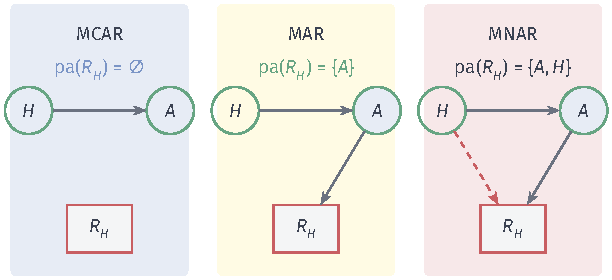
\includegraphics[width=\linewidth]{figures/03-models/03-probabilistic-graphical-models/tikz/pgm-parameter-learning-missingness/figure.pdf}
  \caption{固定已观测的$F,S$后，温度记录指示量$R_H$的三种示意机制。三栏顶部直接给出$R_H$的父集，底部分别配独立日志故障、报警后安排检查、过热改变漏报概率的日常例子。$A$总是观测，$H$在$R_H=0$时不可见；右图需有实际的剩余依赖才属于MNAR，单凭箭头存在不能排除参数抵消。}
  \label{fig:pgm-parameter-learning-missingness}
\end{figure}

\subsection{可忽略性}
\label{sec:pgm-parameter-learning-ignorability}

是否可以不建模$\bm{R}$，要由实际观测的似然判断。对一条记录，令$\bm{y}=(\bm{y}_{\mathrm{obs}},\bm{y}_{\mathrm{mis}})$，在MAR下有
\begin{equation}
  \begin{aligned}
    L(\bm{\theta},\bm{\psi})
      &=\int p_{\bm{\theta}}(\bm{y})
          p_{\bm{\psi}}(\bm{r}\mid\bm{y})
           \,\mathrm{d}\bm{y}_{\mathrm{mis}}\\
      &=p_{\bm{\psi}}(\bm{r}\mid\bm{y}_{\mathrm{obs}})
        p_{\bm{\theta}}(\bm{y}_{\mathrm{obs}}).
  \end{aligned}
  \label{eq:pgm-parameter-learning-ignorability-factorization}
\end{equation}
第二行把不依赖积分变量的机制因子提出。若$\bm{\theta}$与$\bm{\psi}$的参数空间可分离为$\Theta\times\Psi$，即允许任一合法数据参数与任一合法机制参数组合，那么关于$\bm{\theta}$的似然比较不需要机制因子。仅给两组参数起不同名字并不够；若它们受到共同约束，机制仍可能限制$\bm{\theta}$。这里的\term{可忽略性}（ignorability）只表示估计数据参数时可以省略缺失模型，不表示缺失没有损失信息。

基于分布的参数估计还需要适当的先验分离。若$p(\bm{\theta},\bm{\psi})=p(\bm{\theta})p(\bm{\psi})$且相关积分存在，则在MAR下积分掉$\bm{\psi}$只留下与$\bm{\theta}$无关的因子，故$p(\bm{\theta}\mid\bm{y}_{\mathrm{obs}},\bm{r})\propto p_{\bm{\theta}}(\bm{y}_{\mathrm{obs}})p(\bm{\theta})$。若先验把二者关联起来，积分$\int p_{\bm{\psi}}(\bm{r}\mid\bm{y}_{\mathrm{obs}})p(\bm{\psi}\mid\bm{\theta})\,\mathrm{d}\bm{\psi}$一般仍依赖$\bm{\theta}$，不能删除。上述是常用的充分条件，不是每个特定参数问题的必要条件，也不直接等于任意删行或填补程序的有效性保证\scite{pgm-parameter-learning-rubin1976}

\subsection{可忽略缺失下复用未观测变量方法}
\label{sec:pgm-parameter-learning-ignorable-methods}

在可忽略条件下，可以把每条记录实际可见的部分作为$\bm{x}_j=\bm{y}_{j,\mathrm{obs}}$，把缺失部分作为$\bm{z}_j=\bm{y}_{j,\mathrm{mis}}$，直接复用第~\ref{sec:pgm-parameter-learning-latent}节的观测似然、梯度恒等式、精确EM或近似E步。模型若还含主动设置的潜变量$\bm{h}_j$，就把未观测量合并为$\bm{z}_j=(\bm{y}_{j,\mathrm{mis}},\bm{h}_j)$；不同记录可以有不同缺失模式，但每次推断都必须固定该记录实际观测到的分量。

这种映射只复用工具，不把缺失值重新定义为潜变量。删去不完整记录会改变实际使用的数据分布，单次均值填补会忽略条件方差，把缺失值硬填为后验众数也不是EM的E步。对离散模型，应计算相关家庭事件的后验期望计数；对高斯模型，还需二阶矩与交叉矩。若采用摊销推断，识别模型还必须接收缺失掩码或等价的观测模式信息，不能把填充值本身误当成真实观测。

\subsection{不可忽略缺失与可识别性}
\label{sec:pgm-parameter-learning-mnar}

MNAR时，记录过程在给定已观测值后仍依赖缺失值，式~\eqref{eq:pgm-parameter-learning-ignorability-factorization}通常不能分解。此时应为
\[
  p_{\bm{\theta},\bm{\psi}}(\bm{y},\bm{r})
  =p_{\bm{\theta}}(\bm{y})
   p_{\bm{\psi}}(\bm{r}\mid\bm{y})
\]
建立联合模型，把$\bm{R}$作为已观测变量，并对$\bm{Y}_{\mathrm{mis}}$以及原有潜变量共同边缘化。给定这个联合模型后，仍可使用第~\ref{sec:pgm-parameter-learning-latent}节的优化与推断工具；改变的是被拟合的联合分布和待估参数，而不是另造一套EM公式。

联合建模并不自动解决可识别性。不同的数据分布与缺失机制可能诱导同一个$p(\bm{y}_{\mathrm{obs}},\bm{r})$，仅凭现有记录便无法区分它们。对未观测值怎样改变缺失概率的假设，需要由随访数据、外部测量、有效工具变量、受控采集设计或明确的参数约束提供额外信息；缺少这些信息时，应报告敏感性分析，而不能把某个MNAR模型的点估计当作由数据唯一确定的答案。EM只解决给定模型后的计算，不会使不可忽略机制变得可忽略，也不会创造不存在的识别信息。

\section{基于分布估计的参数学习}
\label{sec:pgm-parameter-learning-bayesian}

本节所说\term{分布估计}，专指估计并保留参数后验$p(\bm{\theta}\mid\mathcal{D})$，而不是计算固定参数下模型变量的边缘或后验分布。它与前面三种数据可见性设定交叉：无未观测变量且满足共轭条件时可能解析更新；含潜变量或缺失值时通常要联合近似参数与未观测变量；得到参数后验后，再通过后验预测把参数不确定性传给新数据。

\subsection{不含未观测变量的共轭后验}
\label{sec:pgm-parameter-learning-conjugacy}

不含未观测变量时，局部统计量不仅能用来找最优点，也能更新参数分布。\term{共轭先验}（conjugate prior）是与似然相乘后仍留在同一分布族中的先验，因此可以用有限组超参数记录整个后验，而不必每次做高维积分。

对一个独立参数块$\bm{\eta}$，假设其似然中与参数有关的部分具有形式
\[
  p(\mathcal{D}_b\mid\bm{\eta})
  \propto\exp\{\bm{\eta}^\top\bm{S}_b-n_ba(\bm{\eta})\},
\]
其中$\bm{S}_b$是聚合充分统计量，$n_b$是该块的观测次数，$a$是对应对数归一化函数。若采用相对于指定参数测度、可归一化的先验$p(\bm{\eta}\mid\bm{\chi},\nu)\propto\exp\{\bm{\eta}^\top\bm{\chi}-\nu a(\bm{\eta})\}$，则
\begin{equation}
  p(\bm{\eta}\mid\mathcal{D}_b)
  \propto
  \exp\{\bm{\eta}^\top(\bm{\chi}+\bm{S}_b)
                 -(\nu+n_b)a(\bm{\eta})\}.
  \label{eq:pgm-parameter-learning-conjugate-update}
\end{equation}
指数相加给出$\bm{\chi}\leftarrow\bm{\chi}+\bm{S}_b$与$\nu\leftarrow\nu+n_b$。这一写法适用于拥有共同归一化函数的参数块，例如离散CPT的一行；一般条件指数族的归一化函数可能依赖每条记录的父节点值，不能不看设计条件就把它们都写成$n_ba(\bm{\eta})$。

在所有节点均已观测、没有参数共享且先验也按节点和CPT行独立分解时，似然的分解使后验同样局部分解：
\begin{equation}
  p(\bm{\theta}\mid\mathcal{D})
   =\prod_{i,a}
     \operatorname{Dirichlet}
       (\bm{\theta}_{i,a};
        \bm{\alpha}_{i,a}+\bm{N}_{i,a}).
  \label{eq:pgm-parameter-learning-local-posterior}
\end{equation}
数据沿图结构的作用在这里很具体：每条记录只给各节点家庭的相应单元格增加计数。父配置从未出现时，该行后验仍等于先验，并不是一行由数据支持的精确概率。对完整的线性高斯局部回归，适当的正态与逆Gamma联合先验也可以利用设计矩阵的交叉乘积解析更新，原理同样是聚合局部充分统计量\scite{pgm-murphy2012}

狄利克雷后验保留了整行概率的不确定性，而不只给出式~\eqref{eq:pgm-parameter-learning-cpt-map}的众数。记$\alpha_{i,a,0}=\sum_k\alpha_{i,a,k}$，则
\begin{equation}
  \mathbb{E}[\theta_{i,a,k}\mid\mathcal{D}]
    =\frac{N_{i,a,k}+\alpha_{i,a,k}}
            {N_{i,a}+\alpha_{i,a,0}}.
  \label{eq:pgm-parameter-learning-dirichlet-estimates}
\end{equation}
这个后验均值只需正超参数便定义良好，但它是把参数后验再压缩为一个点，不能代替分布本身。均匀狄利克雷先验下，式~\eqref{eq:pgm-parameter-learning-cpt-map}的内部MAP与MLE相同，常见的加一平滑则来自本式的后验均值。

后验是否局部分解取决于似然和先验共同的结构。共享超参数会将原来独立的块联系起来，缺失数据的求和也通常打破式~\eqref{eq:pgm-parameter-learning-local-posterior}。因此，把EM某一轮的期望计数直接当作真实计数，再宣称获得了精确狄利克雷参数后验，是不正确的。EM固定的是一个参数点，并没有积分该点周围的参数不确定性；完整的贝叶斯处理应针对$p(\bm{\theta},\bm{z}_{1:n}\mid\mathcal{D})$推断。

设备例子也能展示后验保留了多少信息。表~\ref{tab:pgm-parameter-learning-device-counts}给出$5$次故障和$15$次正常，结合$\operatorname{Beta}(2,2)$先验得到$\pi\mid\mathcal{D}\sim\operatorname{Beta}(7,17)$。同一份数据的MLE、MAP与后验均值分别为$1/4$、$3/11$和$7/24$；前两者是不同目标的最优点，第三个数只是后验的一项摘要。该后验的方差为
\[
  \operatorname{Var}(\pi\mid\mathcal{D})
   =\frac{7\times17}{24^2\times25}
   =\frac{119}{14400}\approx0.008264.
\]
这份后验仍有明显宽度，不能把$7/24$解释为已知的真实故障率。新增完整记录后，相应成功或失败计数继续累加即可；先验超参数是建模选择，不应伪装成实测样本。

\subsection{含未观测变量的近似后验}
\label{sec:pgm-parameter-learning-approximate-posterior}

一旦含有潜变量或缺失值，参数后验通常要与未观测变量联合推断；非共轭局部模型和复杂参数共享还会进一步破坏解析形式。此时可以沿用第~\ref{chap:pgm-variational}章和第~\ref{chap:pgm-sampling}章的方法，但必须把推断对象由“固定参数下的状态”扩展为“参数与状态”。以下用$\bm{z}_{1:n}$统称各条记录中的潜变量和实际缺失字段。对MNAR，$\mathcal{D}$还包含已观测的缺失指示，缺失机制参数$\bm{\psi}$也属于联合后验；为显式保留这一情形，下面的公式写出$\bm{\psi}$，不含缺失机制或机制可忽略时则删去所有$\bm{\psi}$项。

变分方法选取$q_{\bm{\phi}}(\bm{\theta},\bm{\psi},\bm{z}_{1:n})$，优化
\begin{equation}
  \begin{aligned}
    \mathcal{L}(\bm{\phi})
      &=\mathbb{E}_{q_{\bm{\phi}}}
       [\log p(\mathcal{D},\bm{z}_{1:n},\bm{\theta},\bm{\psi})
        -\log q_{\bm{\phi}}
          (\bm{\theta},\bm{\psi},\bm{z}_{1:n})],\\
    \log p(\mathcal{D})
      &=\mathcal{L}(\bm{\phi})
        +\operatorname{KL}\bigl(
          q_{\bm{\phi}}\,\|\,
          p(\bm{\theta},\bm{\psi},\bm{z}_{1:n}\mid\mathcal{D})
        \bigr).
  \end{aligned}
  \label{eq:pgm-parameter-learning-bayesian-elbo}
\end{equation}
这里数据参数$\bm{\theta}$与机制参数$\bm{\psi}$的先验都已进入联合分布，两者也都在证据中被积分；$\log p(\mathcal{D})$在模型和超参数固定时是常数。不含$\bm{\psi}$时，公式退化为只对数据参数与状态推断。这个目标与变分EM中随$\bm{\theta}$变化的观测对数似然下界不是同一个优化问题。常用因子化假设可以降低计算量，却可能遗漏参数间相关性或后验的多个峰；优化下界成功不等于近似族已经足够表达真实后验。

在共轭的变分更新中，期望计数确实可能作为超参数出现，但那属于特定变分族下的坐标更新。相应局部状态更新通常使用$\exp\{\mathbb{E}[\log\theta_{i,a,k}]\}$，而不是把后验均值代入$\theta$；一般有$\mathbb{E}[\log\theta]\ne\log\mathbb{E}[\theta]$。这一差别也说明，EM、贝叶斯变分推断与简单的平滑计数不能只凭公式外观互相替代。

MCMC则构造以参数后验或参数与潜变量联合后验为平稳分布的链，用其样本近似积分。若只关心普通可计算似然，后验中与参数无关的证据常数会在Metropolis--Hastings比率中约掉；无向模型的$Z(\bm{\theta})$却依赖候选参数，通常不会消失。这类模型可能仍需额外的内层推断或专门的采样构造。链的混合、多峰之间的移动和有效样本量都需要诊断，不能把“使用MCMC”当作有限运行已得到精确后验的保证。

若后验在一个内部峰附近集中，还可以用\term{拉普拉斯近似}（Laplace approximation），即用峰值附近的二次曲率构造高斯分布。记$g(\bm{\theta})=\log p(\bm{\theta}\mid\mathcal{D})$，在局部MAP点$\widehat{\bm{\theta}}$作二阶展开；若$\bm{H}=-\nabla^2g(\widehat{\bm{\theta}})$正定，则
\[
  p(\bm{\theta}\mid\mathcal{D})
    \approx\mathcal{N}(\bm{\theta};
          \widehat{\bm{\theta}},\bm{H}^{-1}).
\]
边界峰、明显偏斜、多峰或不可识别方向会破坏这一局部高斯描述。对有约束的参数，宜先选择适当坐标，并将密度变换的Jacobian纳入目标；否则曲率和MAP的含义都会改变。三类方法都应通过任务相关的后验量或预测量比较，而不只比较优化器是否停止。

\subsection{后验预测}
\label{sec:pgm-parameter-learning-posterior-predictive}

得到参数后验后，新设备的状态仍具有随机性，而故障率本身也不完全确定。\term{后验预测}（posterior predictive）将这两种不确定性合并：在每个可能参数下计算新观测的分布，再按参数后验加权，
\begin{equation}
  p(\bm{x}_*\mid\mathcal{D})
   =\int p_{\bm{\theta}}(\bm{x}_*)
            p(\bm{\theta}\mid\mathcal{D})\,\mathrm{d}\bm{\theta}.
  \label{eq:pgm-parameter-learning-posterior-predictive}
\end{equation}
若预测还涉及新潜变量，应在内层同时消去它们。\term{插件预测}（plug-in prediction）则把某个点估计$\widehat{\bm{\theta}}$代入$p_{\bm{\theta}}(\bm{x}_*)$，计算较简单，但忽略了参数分布的宽度。

对单台设备的Bernoulli故障变量，后验预测恰好等于代入后验均值的结果：$p(F_*=1\mid\mathcal{D})=\mathbb{E}[\pi\mid\mathcal{D}]=7/24$。这只是概率对$\pi$线性的特例，不说明两种方法一般相同。考虑两台在给定$\pi$后独立的新设备，则
\[
  \begin{aligned}
    p(F_{*,1}=1,F_{*,2}=1\mid\mathcal{D})
      &=\mathbb{E}[\pi^2\mid\mathcal{D}]
        =\frac{7\times8}{24\times25}
        =\frac{7}{75},\\
    p_{\mathrm{plug}}(F_{*,1}=1,F_{*,2}=1)
      &=(7/24)^2=\frac{49}{576}.
  \end{aligned}
\]
两者约为$0.09333$和$0.08507$，相差$\operatorname{Var}(\pi\mid\mathcal{D})$。积分共同参数后，两台设备不再后验预测独立：它们都受到同一故障率未知性的影响。对未来$m$台设备的故障数，完整预测是Beta--二项分布，而非直接代入平均故障率的二项分布。

条件预测还要说明新输入怎样被处理。纯条件模型把$\bm{x}_*$视为给定设计，使用$\int p_{\bm{\theta}}(\bm{y}_*\mid\bm{x}_*)p(\bm{\theta}\mid\mathcal{D})\,\mathrm{d}\bm{\theta}$。若训练的是联合生成模型，新输入本身也能提供参数信息，则严格的条件后验预测为
\[
  p(\bm{y}_*\mid\bm{x}_*,\mathcal{D})
  =\frac{\int p_{\bm{\theta}}(\bm{x}_*,\bm{y}_*)
                      p(\bm{\theta}\mid\mathcal{D})\,\mathrm{d}\bm{\theta}}
         {\int p_{\bm{\theta}}(\bm{x}_*)
                      p(\bm{\theta}\mid\mathcal{D})\,\mathrm{d}\bm{\theta}}.
\]
等价地，它用$p(\bm{\theta}\mid\mathcal{D},\bm{x}_*)$加权条件分布。只有在输入不更新相关参数等条件下，才能直接改用训练后的参数后验作权重。预测对象不同，所需的积分顺序与权重也可能不同。

\section{学习算法分析}
\label{sec:pgm-parameter-learning-analysis}

\subsection{学习与推断的耦合}
\label{sec:pgm-parameter-learning-inference-coupling}

前面各节的差别现在可以落实为学习时缺少哪一种统计量。观测完整且不含潜变量的有向图已经给出局部事件，独立参数块只需聚合计数或回归矩；联合无向图虽然观测完整，仍需计算全局归一化带来的模型期望；条件无向图需要对每个输入计算输出条件分布的期望；含潜变量或缺失值时，还要计算每条记录条件下的后验期望。若联合无向图同时含有潜变量，两类推断任务会同时存在。

例如，对充分统计量为$\bm{T}(\bm{x},\bm{z})$的无向指数族潜变量模型，平均观测似然梯度为
\begin{equation}
  \begin{aligned}
    \frac{1}{n}\nabla_{\bm{\theta}}\ell
      &=\frac{1}{n}\sum_{j=1}^n
        \mathbb{E}_{p_{\bm{\theta}}(\bm{Z}\mid\bm{x}_j)}
          [\bm{T}(\bm{x}_j,\bm{Z})]\\
      &\quad-\mathbb{E}_{p_{\bm{\theta}}(\bm{X},\bm{Z})}
          [\bm{T}(\bm{X},\bm{Z})].
  \end{aligned}
  \label{eq:pgm-parameter-learning-two-expectations}
\end{equation}
第一项问的是“这条观测记录可能来自哪些状态”，第二项问的是“模型不附加证据时会产生哪些状态”。二者不能使用同一组条件样本混为一谈。E步即使容易，M步若含难算的配分函数，也未必容易。

推断复杂度取决于图结构，而不只取决于参数个数。离散完整有向图可以一次扫描累加家庭计数，但表格存储量约为$\sum_i r_i\prod_{v\in\operatorname{pa}(i)}r_v$，高入度节点仍可能很贵。对最大状态数为$r$、诱导宽度为$w$的离散精确消元，主要因子运算规模通常含$r^{w+1}$；潜变量学习还要针对不同证据重复或批量复用这些运算。图固定时可以复用消元结构与消息调度，但参数更新后消息数值一般需要重算。相关算法见第~\ref{chap:pgm-elimination}章和第~\ref{chap:pgm-junction-tree}章。

\subsection{优化与可扩展性}
\label{sec:pgm-parameter-learning-scalability}

当样本数很大时，每次遍历全部记录的代价可能超过单次推断。\term{随机梯度}（stochastic gradient）从小批量记录估计全数据梯度。若优化平均对数似然，大小为$b$的均匀小批量$\mathcal{B}$给出$b^{-1}\sum_{j\in\mathcal{B}}\nabla\log p_{\bm{\theta}}(\bm{x}_j)$；若优化总和目标，则相应乘以$n$。先验项不随样本数重复累加，因而从总和切到均值目标时，正则项也必须同步除以$n$，否则实际上改变了先验相对于数据的强度。

小批量能减少经验项计算，却不会自动解决模型期望或后验推断的偏差。可把实际更新使用的梯度写成
\[
  \widehat{\bm{g}}^{(t)}
   =\nabla J(\bm{\theta}^{(t)})
      +\bm{b}_{\mathrm{inf}}^{(t)}
      +\bm{\xi}^{(t)},
\]
其中$\bm{b}_{\mathrm{inf}}^{(t)}$表示近似推断带来的系统偏差，$\bm{\xi}^{(t)}$表示中心化后的抽样波动。增加小批量大小主要降低波动，不能一般地消去固定步数链或受限变分族的偏差。偏差还可能随着参数改变，因此即使训练曲线平滑，也未必在逼近原来的似然驻点。

参数共享可以显著减少需要估计的自由度，并让罕见局部配置借助其他位置的数据。但共享后，式~\eqref{eq:pgm-parameter-learning-dag-likelihood}虽仍是局部项之和，同一参数的梯度要从所有出现位置累加。关系模板在一条大图上重复出现，也不使这些位置自动成为独立样本；应区分独立设备、独立序列和同一图内部的相关实例。

\term{自动微分}（automatic differentiation）按照计算图的链式法则求导，能够处理共享参数和复杂局部网络，却不会替作者选择正确的统计目标。若反向传播穿过固定次数的消息更新，得到的是该有限计算过程的导数，不一定是精确似然的导数。EM的M步则应固定E步分布，对$Q$中的新参数求导；若无意中让梯度穿过旧后验的构造，就改变了更新的含义。自动微分减少代数实现错误，不能补足不准确的归一化或后验期望。

非凸点估计还依赖初始化。不同初值可能把EM、变分学习或一般梯度法送入不同的吸引区域，多次初始化可以比较实际目标值和预测表现，却不能保证已经发现全局最优。潜变量后验越不确定，参数与期望统计量之间的相互调整还可能越缓慢；只看参数变化小，可能把缓慢移动误判为求解充分。

优化目标本身也可能没有有限最大值。高斯混合模型中，若一个$m$维分量保持固定正权重，把均值移到某个样本$\bm{x}_j$上，并令协方差为$\varepsilon^2\bm{I}$，该点密度正比于$\varepsilon^{-m}$。只要其他分量仍给其余样本正密度，令$\varepsilon\to0$就可使总似然无界。这种\term{退化解}（degenerate solution）来自目标与可行域的边界，不是多运行几轮或更换优化器就能消除。对协方差加下界或采用适当先验可以排除相应路径，但这会改变原来的无约束MLE问题。

评价一个学习流程的误差时，至少要分清三个来源。\term{统计误差}（statistical error）来自有限数据，即使精确求出样本目标的最优解，也未必接近总体最优参数；\term{推断误差}（inference error）来自近似边缘、期望或积分；\term{优化误差}（optimization error）则是相对于所选目标尚未充分求解的差距。模型族不包含真实分布还会产生模型设定偏差，这不能归入优化失败。三类误差未必在参数空间中简单相加，但这个区分可以指导投入：更多数据针对统计不确定性，更准确的内层推断针对近似偏差，更多优化步数只针对当前目标的求解不足。

\subsection{学习结果的评价}
\label{sec:pgm-parameter-learning-evaluation}

\term{不可识别性}（non-identifiability）应在解释参数结果之前检查：若不同参数对应同一个观测分布，数据即使无限多也不能从这些参数中唯一选择一个。交换混合分量的编号并同时交换其权重与局部参数，观测分布不变，这称为\term{标签交换}（label switching）；因子模型的某些旋转、无向势函数的常数重分配以及MNAR模型中数据分布与缺失机制的抵消也会产生不唯一性。约束可以选定一个代表，外部信息可能恢复识别，但增加优化步数不能区分本来观测等价的参数。评价时应优先报告可识别的预测量或与重标记无关的结构，而不是把任意一个参数代表解释为唯一真实机制。

训练似然提高，只说明模型给参与拟合的整批记录分配了更高的概率或密度；条件模型则是在给定输入下提高训练输出的条件似然。若监测的是MAP、ELBO或替代准则，该目标改善并不保证数据似然提高。要判断概率模型能否预测新记录，应使用未参与训练和调参的独立测试集；记录具有分组或时间依赖时，划分也应避免同一设备或未来信息泄漏到训练侧。测试平均预测对数似然可以写为
\[
  \frac{1}{n_{\mathrm{test}}}
  \sum_{j=1}^{n_{\mathrm{test}}}
    \log p_{\mathrm{pred}}(\bm{x}^{\mathrm{test}}_j).
\]
条件模型应改用对应的条件预测概率，缺失数据应使用实际观测部分的概率及所声明的缺失机制。联合分数与条件分数考察的对象不同，不能不加说明地横向比较；连续密度的数值还依赖坐标和单位。

若评估时只能计算ELBO，它报告的是预测对数似然的下界，不是同一个量的精确值。不同模型或不同近似族的下界间隙可能不同，排名也可能受到影响。无向模型若仍未估计$Z$，未归一化能量不能当作对数概率；伪似然或CD训练指标也不能直接代替归一化的测试似然。报告应说明归一化、积分或采样近似所用的方法与误差来源。

对数似然衡量整份概率分配，还可以单独检查概率是否与实际频率吻合。\term{概率校准}（probability calibration）要求预测某事件概率约为$u$的记录中，该事件发生比例也约为$u$。对故障预测，可在独立记录上按预测概率分箱，比较每箱平均概率与故障频率，并同时报告箱内样本量或不确定性。稀疏箱中的偏差不宜直接解释为系统性失准；全部预测一个总体故障率也可能校准，却无法区分高风险与低风险设备。因而校准与区分能力、预测对数似然应结合考察。

参数后验还支持更有针对性的模型检查。\term{后验预测检查}（posterior predictive check）从后验预测中生成与原数据设计相同的重复数据，再比较具有实际意义的统计量。例如，设备模型可以比较总报警率、各故障组的过热率，以及给定$H,S$后报警与故障之间是否仍有模型没有解释的关联。若研究对象包含缺失过程，复制数据时也应模拟相应记录机制，或明确固定了什么观测设计。观测统计量长期落在预测分布的边缘，提示模型结构、局部分布或先验可能不适合当前数据。

后验预测检查是诊断模型与数据的不相容之处，不能把同一批数据参与拟合后的吻合程度当作独立泛化证据，也不能把没有发现问题当作模型已经正确。积分参数得到的模型证据、比较两个证据之比的Bayes因子，以及BIC，主要服务于模型或结构比较，且需要考虑先验与正则条件。第~\ref{sec:pgm-structure-learning-scores}节将给出它们的定义，并说明这种比较与参数拟合、预测评价的区别。

\section{本章小结}
\label{sec:pgm-parameter-learning-summary}

参数学习由数据可见性与参数估计方式两条轴共同决定。前者区分无潜变量的完整观测、含潜变量的完整观测和字段缺失，决定能否直接取得统计量、是否需要边缘化或建模缺失机制；后者区分MLE、MAP点估计与保留参数后验的分布估计。两轴可以组合，潜变量、缺失值、非共轭性和全局归一化都可能使两类估计依赖近似推断。

算法保证取决于目标。精确EM在精确E步、充分M步下保证观测似然不下降；广义EM保留精确E步，M步只须改善同一$Q$函数。变分EM仅当两步都改善同一ELBO时，才保证该下界不下降；有限样本Monte Carlo E步没有统一的逐轮ELBO或观测似然单调保证。Wake--Sleep优化不同方向的目标，不保证观测似然或真实数据ELBO逐轮改善。评价还须区分三类误差，检查初始化、退化边界与不可识别性。
